\chapter{TINJAUAN PUSTAKA}\label{bab-ii-tinjauan-pustaka}

\section{Dasar Teori}\label{dasar-teori}

Pada bagian ini, akan dijelaskan beberapa teori yang digunakan dalam penelitian ini terkait dengan pengujian perangkat lunak otomatis, teknik yang digunakan, serta alat-alat yang mendukung penelitian ini. Setiap teori dijelaskan secara mendalam untuk menunjukkan bagaimana teori tersebut digunakan dalam konteks pengujian aplikasi berbasis web menggunakan TathyaTest.

\subsection{Pengujian Perangkat Lunak}\label{pengujian-perangkat-lunak}

Pengujian perangkat lunak adalah suatu proses yang bertujuan untuk memastikan bahwa perangkat lunak berfungsi sesuai dengan spesifikasi yang telah ditetapkan dan bebas dari kesalahan. Software testability, yaitu kemampuan perangkat lunak untuk mendukung pengujiannya sendiri, menjadi faktor penting dalam menentukan efektivitas proses pengujian \parencite{garousi2019testability}. Pengujian ini juga bertujuan untuk memastikan aplikasi dapat berjalan dengan baik dalam berbagai kondisi, baik itu dalam kondisi normal maupun saat terjadi lonjakan jumlah pengguna.

Dalam konteks aplikasi berbasis web, pengujian bertujuan untuk memastikan aplikasi dapat beroperasi dengan baik di berbagai platform dan perangkat. Di Jurusan Teknologi Informasi, aplikasi berbasis web sering digunakan untuk pengelolaan data akademik dan administrasi, sehingga kualitas pengujian menjadi sangat penting untuk memastikan fungsionalitas aplikasi yang maksimal.

Pengujian perangkat lunak juga penting untuk mendeteksi masalah yang mungkin muncul selama penggunaan aplikasi, misalnya kegagalan dalam proses CRUD (Create, Read, Update, Delete), autentikasi pengguna, dan akses modul \parencite{wang2023}. Oleh karena itu, pengujian yang menyeluruh sangat dibutuhkan agar aplikasi dapat berfungsi dengan baik sesuai harapan.

\subsection{Automation Testing}\label{automation-testing}

Automation testing adalah pendekatan yang memungkinkan pengujian perangkat lunak dilakukan secara otomatis tanpa intervensi manusia. Dalam konteks pengembangan perangkat lunak modern, automated testing memberikan berbagai peluang untuk meningkatkan efisiensi dan kualitas, namun juga menghadirkan tantangan yang perlu dikelola dengan baik, seperti kompleksitas implementasi, maintenance overhead, dan integrasi dengan proses development \parencite{solige2025automation}. Keunggulan utama dari otomatisasi adalah penghematan waktu, karena pengujian dapat dilakukan berulang kali tanpa menambah beban kerja. Selain itu, otomatisasi juga mengurangi kesalahan manusia, yang sering kali terjadi dalam pengujian manual.

Dalam penelitian ini, TathyaTest menggunakan pendekatan automation testing untuk mengotomatisasi pengujian aplikasi berbasis web yang digunakan oleh mahasiswa dan dosen. Pengujian dilakukan dengan menggunakan alat seperti Playwright, yang berdasarkan analisis komparatif terbaru menunjukkan efektivitas superior dalam hal waktu eksekusi dan penggunaan resource dibandingkan tools lain seperti Cypress dan Selenium \parencite{mon2025}.

Keuntungan lainnya adalah pengujian berulang dapat dilakukan tanpa memerlukan sumber daya tambahan, membuat proses pengujian lebih efisien dalam hal waktu dan biaya. Automation testing juga memungkinkan pengujian dilakukan dalam skala besar dan dengan cakupan yang lebih luas, yang mana akan sangat berguna dalam pengujian aplikasi berbasis web yang kompleks \parencite{shah2021}.

\subsection{Crawling URL}\label{crawling-url}

Crawling URL adalah teknik yang digunakan untuk menjelajahi halaman aplikasi berbasis web secara otomatis dan mengumpulkan informasi penting dari halaman-halaman tersebut \parencite{mishra2020}. Proses ini memanfaatkan teknik web crawling untuk mengidentifikasi elemen-elemen yang perlu diuji, seperti formulir input, tombol, dan tabel data. Pada aplikasi web modern yang banyak memanfaatkan rendering sisi klien (client-side rendering), termasuk aplikasi single-page application (SPA) berbasis React, crawler berbasis HTML statis tidak dapat menjangkau elemen yang baru muncul setelah DOM dirender oleh browser; oleh karena itu diperlukan pendekatan crawling yang menjelajahi DOM yang telah ter-render sepenuhnya \parencite{mesbah2012crawljax}. Dengan menggunakan crawling semacam ini, TathyaTest direncanakan dapat secara otomatis mengakses halaman-halaman aplikasi dan mengidentifikasi elemen-elemen pengujian yang relevan untuk pengujian lebih lanjut, termasuk pada aplikasi yang dikendalikan akses per peran pengguna (RBAC).

Melalui crawling, TathyaTest direncanakan dapat menavigasi aplikasi web dan mengumpulkan data penting untuk pembuatan test case otomatis \parencite{leotta2021}. Hal ini memungkinkan alat untuk mendeteksi berbagai elemen interaktif yang ada di aplikasi, tanpa perlu pengaturan manual yang memakan waktu. Dengan crawling yang efisien, alat ini dapat menghemat waktu dalam mempersiapkan data yang diperlukan untuk pengujian, sehingga lebih banyak skenario pengujian dapat dilakukan.

\subsection{Ekstraksi Elemen HTML}\label{ekstraksi-elemen-html}

Setelah melakukan crawling, langkah berikutnya adalah mengekstrak elemen-elemen HTML yang ditemukan pada halaman web yang telah di-crawl. Perkembangan teknik web data extraction, termasuk pendekatan berbasis machine learning, telah membuat proses ekstraksi data dari halaman web menjadi lebih efisien dan adaptif \parencite{patnaik2021}. Ekstraksi elemen HTML sangat penting untuk memperoleh elemen-elemen seperti formulir input, tombol, tautan, dan tabel yang diperlukan untuk pengujian fungsional aplikasi. Karena DOM yang relevan hanya tersedia setelah dirender sepenuhnya oleh browser, ekstraksi direncanakan dilakukan langsung pada konteks browser (misalnya melalui skrip evaluasi DOM yang dijalankan pada halaman yang telah ter-render), bukan dengan mem-parsing berkas HTML statis.

Ekstraksi elemen HTML memungkinkan TathyaTest untuk mengidentifikasi elemen-elemen yang dapat diuji dalam aplikasi, seperti elemen interaktif yang berfungsi untuk input data atau navigasi pengguna \parencite{romano2022}. Setelah elemen-elemen ini diidentifikasi, test case otomatis dapat dibuat untuk menguji fungsionalitas masing-masing elemen. Proses ekstraksi ini juga memastikan bahwa cakupan pengujian lebih luas, mencakup semua elemen yang ada di aplikasi, baik yang terlihat maupun yang tersembunyi.

\subsection{Playwright}\label{playwright}

Playwright adalah alat pengujian otomatis berbasis JavaScript yang dirancang untuk menguji aplikasi web secara end-to-end. Studi komparatif terbaru menunjukkan bahwa Playwright unggul dalam performa dibandingkan dengan Cypress dan Selenium, khususnya dalam hal waktu eksekusi, penggunaan CPU, dan konsumsi RAM \parencite{mon2025}. Salah satu keunggulan Playwright adalah kemampuannya untuk melakukan cross-browser testing, yang memungkinkan pengujian dilakukan di berbagai browser seperti Chrome, Firefox, dan WebKit dengan hasil yang konsisten. Hal ini sangat berguna untuk memastikan aplikasi berfungsi dengan baik di berbagai platform.

Dalam penelitian ini, Playwright digunakan untuk mengeksekusi test case otomatis yang dihasilkan oleh TathyaTest setelah proses crawling dan ekstraksi elemen HTML. Dengan Playwright, pengujian dilakukan secara menyeluruh pada berbagai browser untuk memastikan bahwa aplikasi berfungsi dengan baik di semua platform yang digunakan oleh pengguna. Proses test case otomatis ini mengadopsi pendekatan dalam \parencite{sahoo2021}. Pendekatan ini juga memungkinkan untuk melakukan real-time testing, yang mempercepat proses pengujian dan memperbaiki bug secara langsung.

Fitur unggulan lainnya adalah kemampuan Playwright untuk mengontrol browser secara langsung, memungkinkan interaksi dengan elemen-elemen aplikasi dan memverifikasi fungsionalitasnya. Dengan demikian, Playwright menjadi alat yang ideal untuk memastikan bahwa aplikasi web diuji secara menyeluruh dengan akurasi yang tinggi.

\section{State of the Art}\label{state-of-the-art}

Pengujian perangkat lunak, terutama untuk aplikasi berbasis web, adalah langkah penting dalam memastikan kualitas dan keandalan perangkat lunak. Automation testing, yang memungkinkan pengujian dilakukan secara berulang tanpa memerlukan intervensi manusia, telah terbukti meningkatkan efisiensi dan mengurangi kemungkinan kesalahan. Berbagai pendekatan, dari crawling-based testing hingga model-based testing, telah digunakan untuk meningkatkan efektivitas pengujian aplikasi web \parencite{wang2023}.

Salah satu pendekatan yang banyak digunakan adalah test case generation otomatis yang memungkinkan alat pengujian menghasilkan langkah-langkah pengujian secara otomatis berdasarkan elemen-elemen aplikasi. Pendekatan ini dapat meningkatkan cakupan pengujian dan mengidentifikasi skenario pengujian yang mungkin terlewat dalam pengujian manual \parencite{setiani2019}. Selain itu, penelitian terkini menunjukkan pentingnya pemeliharaan test case dalam pengujian otomatis, dengan pendekatan seperti visual web test repair yang memanfaatkan computer vision untuk memperbaiki test case yang rusak akibat perubahan UI aplikasi web \parencite{stocco2018}.

Beberapa penelitian juga menunjukkan bahwa ekstraksi elemen HTML menggunakan teknik seperti selektor CSS dan XPath sangat efektif untuk mengekstrak elemen-elemen penting dari aplikasi berbasis web. Tren terkini dalam web data extraction menunjukkan evolusi dari metode manual ke metode otomatis dan intelligent extraction menggunakan machine learning, yang meningkatkan akurasi dan adaptabilitas sistem ekstraksi \parencite{patnaik2021}. Dengan menggunakan teknik-teknik ini, TathyaTest dapat menghasilkan test case otomatis yang lebih efisien dan lebih menyeluruh.

Secara keseluruhan, penelitian sebelumnya menunjukkan bahwa alat seperti Selenium, Cypress, dan Playwright sangat efektif dalam meningkatkan efisiensi dan efektivitas pengujian perangkat lunak. TathyaTest menggabungkan berbagai teknik ini, dengan fokus pada crawling URL dan ekstraksi elemen HTML untuk menghasilkan test case otomatis yang meningkatkan cakupan pengujian dan memastikan aplikasi diuji dengan menyeluruh.

\section{Roadmap Penelitian}\label{roadmap-penelitian}

Pengembangan penelitian TathyaTest dirancang secara berkelanjutan selama lima tahun untuk memperkuat kontribusi keilmuan di bidang pengujian perangkat lunak otomatis, khususnya pada aplikasi berbasis web. Roadmap ini menggambarkan arah riset strategis yang saling berkelanjutan dan berjenjang sebagai berikut:

\vspace{0.3cm}

\begin{figure}[ht]
\centering
\resizebox{\textwidth}{!}{
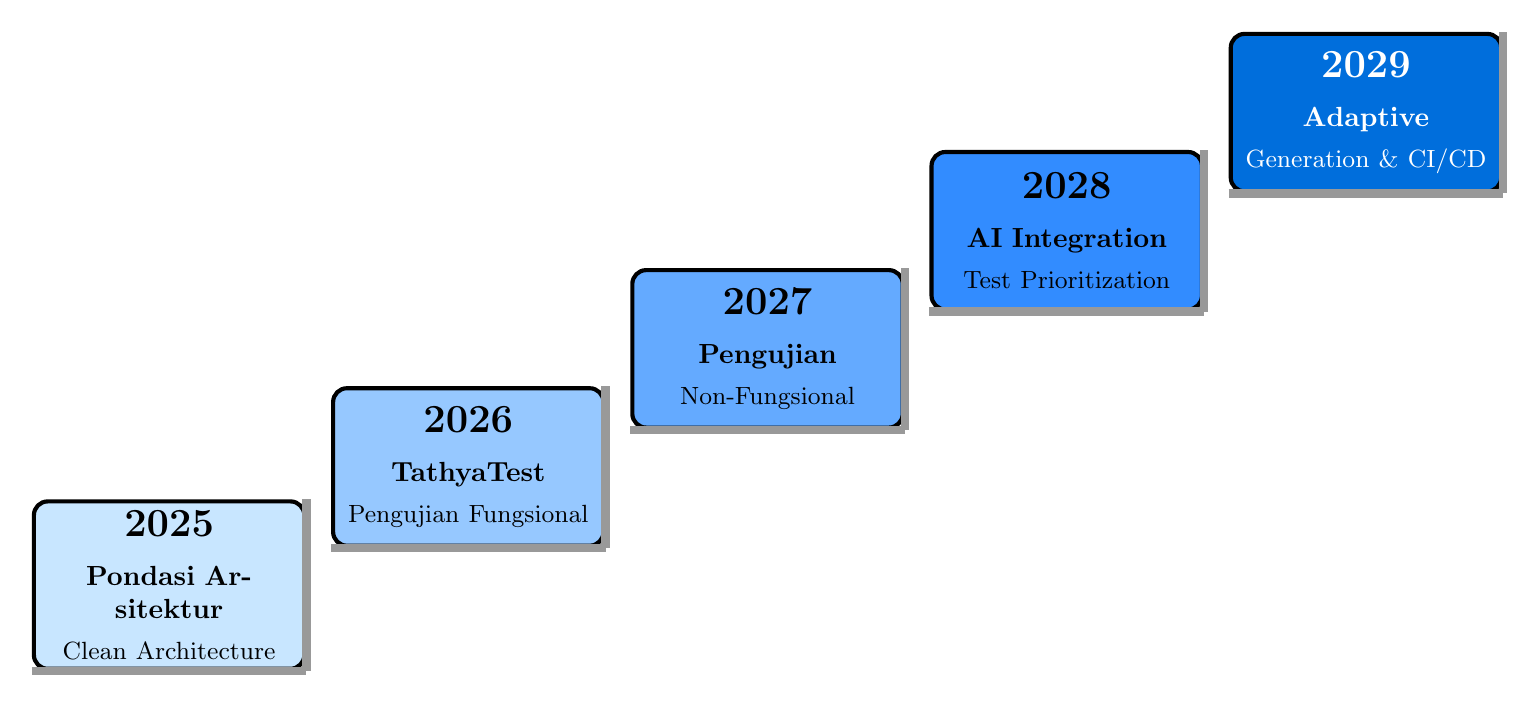
\begin{tikzpicture}[
    every node/.style={align=center},
    stepbox/.style={rectangle, draw=black, line width=1.5pt, text width=3.2cm, minimum height=2cm, rounded corners=5pt}
]

% Define colors for gradient
\definecolor{color1}{RGB}{200, 230, 255}  % Very light blue
\definecolor{color2}{RGB}{150, 200, 255}  % Light blue
\definecolor{color3}{RGB}{100, 170, 255}  % Medium light blue
\definecolor{color4}{RGB}{50, 140, 255}   % Medium blue
\definecolor{color5}{RGB}{0, 110, 220}    % Strong blue

% Step 1 - 2025
\node[stepbox, fill=color1] (s1) at (0,0) {
    \fontsize{14}{16}\selectfont\textbf{2025}\\[0.2cm]
    \normalsize\textbf{Pondasi Arsitektur}\\[0.1cm]
    \small Clean Architecture
};

% Step 2 - 2026
\node[stepbox, fill=color2] (s2) at (3.8,1.5) {
    \fontsize{14}{16}\selectfont\textbf{2026}\\[0.2cm]
    \normalsize\textbf{TathyaTest}\\[0.1cm]
    \small Pengujian Fungsional
};

% Step 3 - 2027
\node[stepbox, fill=color3] (s3) at (7.6,3) {
    \fontsize{14}{16}\selectfont\textbf{2027}\\[0.2cm]
    \normalsize\textbf{Pengujian}\\[0.1cm]
    \small Non-Fungsional
};

% Step 4 - 2028
\node[stepbox, fill=color4] (s4) at (11.4,4.5) {
    \fontsize{14}{16}\selectfont\textbf{2028}\\[0.2cm]
    \normalsize\textbf{AI Integration}\\[0.1cm]
    \small Test Prioritization
};

% Step 5 - 2029
\node[stepbox, fill=color5, text=white] (s5) at (15.2,6) {
    \fontsize{14}{16}\selectfont\textbf{2029}\\[0.2cm]
    \normalsize\textbf{Adaptive}\\[0.1cm]
    \small Generation \& CI/CD
};

% Draw base lines for stairs effect
\draw[line width=3pt, color=black!40] (s1.south west) -- (s1.south east);
\draw[line width=3pt, color=black!40] (s1.south east) -- (s1.north east);

\draw[line width=3pt, color=black!40] (s2.south west) -- (s2.south east);
\draw[line width=3pt, color=black!40] (s2.south east) -- (s2.north east);

\draw[line width=3pt, color=black!40] (s3.south west) -- (s3.south east);
\draw[line width=3pt, color=black!40] (s3.south east) -- (s3.north east);

\draw[line width=3pt, color=black!40] (s4.south west) -- (s4.south east);
\draw[line width=3pt, color=black!40] (s4.south east) -- (s4.north east);

\draw[line width=3pt, color=black!40] (s5.south west) -- (s5.south east);
\draw[line width=3pt, color=black!40] (s5.south east) -- (s5.north east);

\end{tikzpicture}
}
\caption{Roadmap Penelitian TathyaTest 2025-2029}
\label{fig:roadmap}
\end{figure}

\vspace{0.3cm}

\textbf{2025 -- Pondasi Arsitektur: Clean Architecture sebagai Landasan Pengujian}

Pada tahun pertama, penelitian telah difokuskan pada pengembangan arsitektur perangkat lunak yang bersih dan terstruktur sebagai landasan untuk sistem pengujian ke depan. Penelitian tentang implementasi Clean Architecture pada aplikasi web telah dipublikasikan dan menjadi pondasi penting untuk membangun sistem pengujian yang efektif \parencite{rifai2025clean}. Arsitektur yang terstruktur dengan baik memungkinkan identifikasi komponen dan alur pengujian yang lebih jelas, yang akan menjadi dasar pengembangan TathyaTest.

\textbf{2026 -- Implementasi TathyaTest untuk Pengujian Fungsional}

Pada tahun kedua, penelitian ini berfokus pada implementasi TathyaTest sebagai alat test case generator otomatis untuk pengujian fungsional aplikasi berbasis web. Dengan memanfaatkan pondasi Clean Architecture dari tahun sebelumnya, TathyaTest dikembangkan untuk mengidentifikasi elemen-elemen aplikasi dan menghasilkan test case otomatis menggunakan crawling DOM ter-render (Playwright) dan ekstraksi elemen HTML pada konteks browser. Pengujian fungsional akan mencakup operasi CRUD, autentikasi pengguna, dan akses modul, dengan integrasi Playwright untuk cross-browser testing pada Chrome, Firefox, dan WebKit.

\textbf{2027 -- Pengujian Non-Fungsional untuk TathyaTest}

Pada tahun ketiga, fokus penelitian akan berkembang dari pengujian fungsional ke pengujian non-fungsional. TathyaTest akan diperluas untuk dapat menghasilkan test case yang menguji aspek non-fungsional aplikasi, termasuk performance testing untuk mengukur kinerja dan response time, security testing untuk mengidentifikasi kerentanan keamanan, dan load testing untuk mengevaluasi kemampuan aplikasi menangani beban pengguna yang tinggi. Penelitian ini akan mengeksplorasi teknik-teknik otomatis untuk menghasilkan test case non-fungsional yang relevan berdasarkan karakteristik aplikasi.

\textbf{2028 -- Integrasi AI untuk Test Case Prioritization dan Risk Analysis}

Pada tahun keempat, penelitian akan mengintegrasikan kecerdasan buatan (AI) dalam TathyaTest untuk test case prioritization dan risk analysis. Teknik machine learning akan digunakan untuk menganalisis historical test data dan code changes, kemudian memprioritaskan test case berdasarkan tingkat risiko dan probabilitas bug. Penelitian ini akan mengeksplorasi algoritma classification dan regression untuk memprediksi area aplikasi yang rawan bug, sehingga dapat mengoptimalkan urutan eksekusi test case dan mengurangi waktu pengujian dengan tetap mempertahankan cakupan yang efektif.

\textbf{2029 -- Adaptive Test Generation dan Integrasi CI/CD}

Pada tahun kelima, penelitian akan mengembangkan adaptive test generation yang dapat belajar dari hasil pengujian sebelumnya dan menyesuaikan strategi pengujian secara otomatis. Machine learning akan digunakan untuk mengidentifikasi pola kegagalan pengujian dan secara dinamis menghasilkan test case baru untuk area yang belum tercakup. Penelitian ini juga akan mengintegrasikan TathyaTest dengan sistem CI/CD (Continuous Integration/Continuous Deployment) untuk memungkinkan pengujian otomatis berkelanjutan yang cerdas dalam siklus pengembangan perangkat lunak, dengan kemampuan self-healing test yang dapat memperbaiki test case yang rusak akibat perubahan aplikasi.

